\documentclass[10pt]{article}
\usepackage[utf8]{inputenc}
\usepackage[T1]{fontenc}
\usepackage[english]{babel}
\usepackage{amsfonts}
\usepackage{amsmath}
\usepackage[pdftex]{color,graphicx}
\usepackage{fancyhdr}
\usepackage{textcomp}
\usepackage{lmodern}
\usepackage{xcolor}
\usepackage{multicol}
\usepackage{soul}
\usepackage{algorithmic}
\usepackage{wrapfig}
\usepackage{float}
\usepackage{mdwlist}
\usepackage{pgfgantt}
%\usepackage{hyperref}
\pagestyle{fancy}
\newcommand{\HRule}{\rule{\linewidth}{0.5mm}}

%If in need of a header for the document, uncomment this and add desired text!
%\fancyhead[LO,LE]{}
%\fancyhead[RO,RE]{}
%%%%%%%%%%%% END OF PREAMBLE %%%%%%%%%%%%%%%%%%%%%%%%%%%%%%%%%%%%
\begin{document}
\begin{titlepage}

\begin{center}

\textsc{\LARGE DATANET}\\[1.5cm]

%\textsc{\Large Datanet}\\[0.5cm]

\HRule \\[0.4cm]

{ \bfseries Weekly assignment 3}\\[1cm]
%\includegraphics[width=0.8\textwidth]{carrie}\\[0.1cm]

\HRule \\ [7.5cm]

% Author and supervisor
\begin{minipage}{0.5\textwidth}
\begin{flushleft} \large
Martin Jørgensen (tzk173)\\
\textit{martinnjorgensen@gmail.com}\\
\end{flushleft}
\end{minipage}
\begin{minipage}{0.4\textwidth}
\begin{flushright} \large
\textbf{\today} \\
\end{flushright}
\end{minipage}

\vfill

% Bottom of the page front page


\end{center}

\end{titlepage}
\clearpage

\section{Theoretical part}

\subsection{The Internet Protocol}
\subsubsection{Addresses and network masks}
\textbf{Part1:}\\
\begin{enumerate*}
  \item The purpose of network masking is to allow the network/internet to
        identify several machines behind a single router using as few addresses
        as possible. It also allows for seperation of networks into different
        blocks (subnets.)
  \item \texttt{255.225.255.0} is a valid subnet mask since \textit{binary-and}
        can still be applied over the mask. \texttt{/28} should be interpreted
        as the 28 most significant bits being one, giving a mask of:
        \texttt{11111111.11111111.11111111.11110000} = \texttt{255.255.255.240}
        giving 16 subnets with 14 hosts each.
  \item Classfull \textit{CIDR} networks allows for only 3 subnet masks:
        \begin{itemize*}
          \item Class A: 8-bit subnet mask or (255.0.0.0)
          \item Class b: 16-bit subnet mask or (255.255.0.0)
          \item Class c: 24-bit subnet mask or (255.255.255.0)
        \end{itemize*}
        Classless allows subnet masks from 0-bit to 32-bit. 32 and 31 bit masks
        being useless though.
  \item The subnet mask itself tells us the IP configuration of the network,
        number of possible subnets, sizes etc. Using the the subnet mask on any
        obtained IP's from the network then allows for the computation of an
        actual internal IP, which can be used to see what subnets are
        "populated".
\end{enumerate*}

\noindent \textbf{Part2:}\\
\begin{enumerate*}
  \item \begin{itemize*}
          \item Subnet Size: 30 hosts
          \item Network address: \texttt{130.225.165.16}
          \item Mask: \texttt{255.255.255.224}
          \item Broadcast address: \texttt{130.225.165.31}
          \item 1st IP: \texttt{130.225.165.1}
          \item 5th IP: \texttt{130.225.165.5}
          \item Last IP: \texttt{130.225.165.30}
        \end{itemize*}

  \item \begin{itemize*}
          \item Subnet Size: 254 hosts
          \item Network address: \texttt{10.0.42.0}
          \item Mask: \texttt{255.255.254.0}
          \item Broadcast address: \texttt{255.255.254.255}
          \item 1st IP: \texttt{255.255.254.1}
          \item 5th IP: \texttt{255.255.254.5}
          \item Last IP: \texttt{255.255.254.254}
        \end{itemize*}

  \item \begin{itemize*}
          \item Subnet Size: 1 host
          \item Network address: \texttt{4.2.2.1}
          \item Mask: \texttt{255.255.255.255}
          \item Broadcast address: N/A only one host.
          \item 1st IP: \texttt{4.2.2.1}
          \item 5th IP: N/A
          \item Last IP: N/A
        \end{itemize*}

  \item \begin{itemize*}
          \item Subnet Size: 16382 hosts
          \item Network address: \texttt{192.38.64.0}
          \item Mask: \texttt{255.255.192.0}
          \item Broadcast address: \texttt{192.38.127.255}
          \item 1st IP: \texttt{192.38.64.1}
          \item 5th IP: \texttt{192.38.64.5}
          \item Last IP: \texttt{192.38.127.254}
        \end{itemize*}
\end{enumerate*}


\subsubsection{Network Address Translation}

\noindent \textbf{Part 1:}\\
The NAT maps all internal addresses(Ip,port) via a translation table so it can
manage the relationships between different internal and external connections. It
maps both IP and port on both sides, allowing different processes from same IP
to work as long as the NAT have available ports.

\noindent \textbf{Part 2:}\\
Since a NAT requires memory for the table racking up a lot of long term
connections can fill up it's memory. another factor is the fact that the port
field is a fixed 16-bits meaning all the ports can be taken up, there is 65535
ports available.

\noindent \textbf{Part 3:}\\
The NAT breaks the layering because it modifies the TCP/UDP headers ,thereby
breaking into the 4th layer (transport).

\subsection{Distributed Hash Tables}
\begin{enumerate*}
  \item \textbf{TODO!}
  \item \textbf{TODO!}
  \item \textbf{TODO!}
\end{enumerate*}

\subsection{SSH Tunneling}

\subsubsection{Part 1}
\noindent \textbf{Q1:}\\
The server is waiting for someone to connect on the "serversock". It is blocked
at line 24 in the \texttt{socket.accept()} call.

\noindent \textbf{Q2:}\\
The port is different because the client socket connects TO port 6789, not from
it. The FROM port is chosen by the system and not the program.

\noindent \textbf{Q3:}\\

I can see the messages because they're not encrypted or encoded in some other
format. TCPdump just picks up the TCP packets coming on port 6789 and prints the
content including TCP header. The content is plaintext, so it shows up in the
terminal.

\subsubsection{Part 2}

\noindent \textbf{Q4:}\\
Í am unable to connect, there can be several reasons for this inability. The Í
most likely is firewalling on DIKU prevent connections on ports that SCIENCE- Í
IT do not use themselves, only allowing outbound connections on these ports.
Also, \texttt{ping} is an \textit{ICMP} packet and not a TCP packet like the
socket connections in python. This means firewall treat the differently, ICMP is
usually allowed. evne if all TCP ports are closed.

\noindent \textbf{Q5:}\\

The important bit is \texttt{6790:localhost:6002} it means that connection on
our loopback interface that targets port 6790 should be directed through the SSH
tunnel to port 6002 on the loopback interface at ask.diku.dk. So as long as both
client and server sends to the loopback interface at the 2 specified ports, they
can "talk" to each other.

\noindent \textbf{Q6:}\\
\textit{TCP dump output attached as q6.txt if needed}\\
I can still see the output, the eason is the same as in Q3, we're sending stuff
to the loopback interface in plaintext, therefore it is readable.

\noindent \textbf{Q7:}\\
Removing the \texttt{-i lo} switch removes the output because my machine
defaults to the eth0 interface, which is not connected. Switching to
\textit{wlan0} also yields nothing since we're talking TO the loopback interface
using port 6790.

\noindent \textbf{Q7.5??:}\\
Using my own public IP I can see a connection from my routers port 37456 to
ask.diku.dk's port 22. Port 22 is commonly used for SSH services.

\noindent \textbf{Q8:}\\
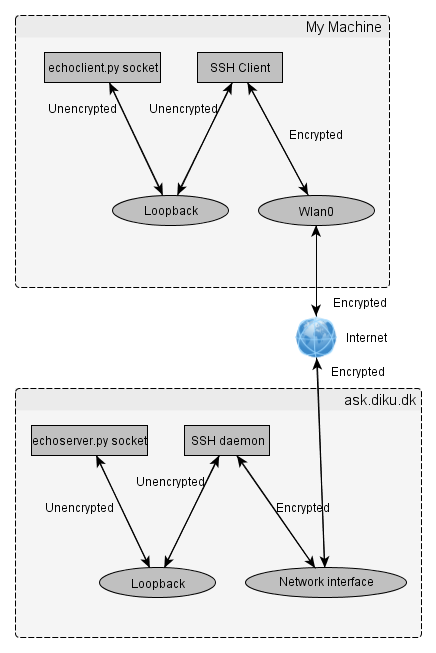
\includegraphics[width=\textwidth]{q8.png}


\section{Practical Section}

\subsection{Question 1}
Since the program currently only listens to localhost (the loopback interface)
any peer NOT on the machine will be unable to connect unless employing some sort
of port forwarding like SSH tunneling.

Assuming a server that listens on an actual network interface and a network with
NO firewall or other obstructions the following communication can take place:
\begin{verbatim}
Peer B <-> NS    : HANDSHAKE
Peer B --> NS    : LOOKUP Peer A
Peer B <-- NS    : INFO ...
Peer B <-> Peer A: HANDSHAKE
Peer B --> Peer A: MSG ...
Peer B <-- Peer A: MSG ACK
\end{verbatim}

\subsection{Question 2}
I personally keep the socket alive, this means that no further handshakes are
required for communicating with any of the present peers. The drawback is of
course that I am blocking system resources that could maybe be used by other
services. closing down sockets after a broadcast would free these resources, but
since this is an academic excersice, and I know that the peers will not be
connected in networks with 100.000s of peers I opted to keep them open.

\subsection{Question 3}
To allow multicasting, I would create a new dict with group ID's (key) and a
list of member nicks (value). The group ID would then be negotiated between the
peers when creating the group, and a new \texttt{GMSG} message implemented that
send the group ID followed by the actual message.

Of course negotiating an ID that is not used can b tough in larger networks, and
this model have drawbacks, if 6 peers create 2 seperate groups of 3 with same
ID, the peers wil lbe unable to join the other groups because the ID for the
dict is already in use.

\subsection{Question 4}

A \textit{divide and conquer} method could be devised, we're the broadcasting
peer once it recieves the userlist, picks a number of the peers and request that
they help broadcasting the message. If the broadcasting peer sends the message
to 2 peers, and the relay it to 2 peers each, the propegation time would be
$O(log(n))$ instead. This means the the prorocal would need to be changed to
allow this new command, and an algorithm for selecting peers that eliminate
double transmissions (two peers write to the same peer) would need to be
devised.

\subsection{Question 5}
We need the \texttt{MSG ACK} because there is no quarentee that the peer we're
talking to as able to show the message, it could use a different format (version
inconsistency?), or the other end might not be a peer at all, but another
program using a similar but not identical protocol. The same goes for
\texttt{BYE}, it means the peer will wait with closing the connection until the
other peer have confirmed that it will remove the first peer from its dicts and
lists.

\end{document}